Grid is the exception in Table~\ref{tab:threshold}: its LOO threshold is so conservative that almost no defect is flagged (recall 1.2\,\%, F1 0.023 for PatchCore-lite), which lowers every five-category mean. On the other four textures PatchCore-lite with $k=10$, $m=0.1$ reaches F1 0.935 at 4.3\,\% FPR and 89.4\,\% recall.

\subsection{Confidence-Gated Offloading}\label{sec:res-gate}
Fig.~\ref{fig:gate} shows the accuracy--offload trade-off obtained by sweeping $\alpha\in[0.3,1]$ for three values of $\beta$, and Table~\ref{tab:gate} details the a-priori operating point. Station-only inspection never offloads but reaches only F1 0.659 with 28.2\,\% false alarms; edge-only inspection reaches F1 0.753 at 3.4\,\% FPR but offloads every frame. The gated cascade with $(\alpha,\beta)=(0.6,1.5)$ attains F1 0.748---99.3\,\% of the edge-only value---while offloading 50.9\,\% of frames, and cuts the station-only false-alarm rate from 28.2\,\% to 7.9\,\%. Excluding grid, the cascade reaches F1 0.930 versus 0.935 for edge-only and 0.801 for station-only. Along the Pareto front, $(\alpha,\beta)=(0.7,1.5)$ keeps F1 at 0.739 with 39.8\,\% offload, and $(0.6,2.0)$ matches edge-only (0.753) with 61.8\,\%; the lower bound of the band, $\alpha$, controls how many frames are trusted as clearly normal and is the dominant knob, whereas $\beta=\infty$ (never declaring defects locally) wastes offloads on frames the station already recognises as defective.

The gate adapts to the fabric automatically (Table~\ref{tab:gate}): it offloads only 23\,\% of leather and 30\,\% of wood frames, where the station model is already strong, but 81\,\% of carpet frames, where it is weak. This is the desired behaviour of an uncertainty-driven policy, and it emerges from the LOO thresholds alone, without any labelled tuning per fabric. It also corrects the station's worst failure, the 95.8\,\% false-alarm rate on leather, to 19.8\,\%. The residual gap to edge-only on leather (FPR 4.2\,\%) comes from frames whose station score exceeds $\beta\tau_g$ although they are defect-free, which a larger $\beta$ removes at the cost of more offloads.

\begin{figure}[t]
\centering
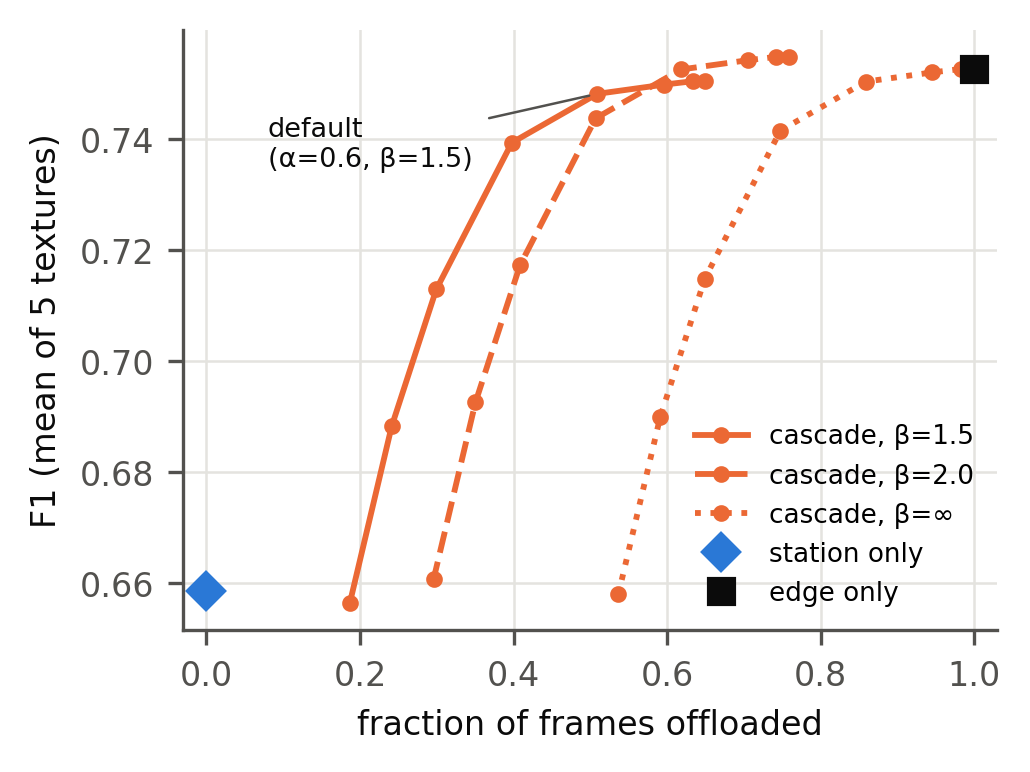
\includegraphics[width=\columnwidth]{fig_gate.png}
\caption{Accuracy--offload trade-off of the gate ($k=10$, mean of five textures and three draws). Each curve sweeps $\alpha$ from 1.0 (left) to 0.3 (right).}
\label{fig:gate}
\end{figure}

\begin{table}[t]
\centering
\caption{Per-fabric decisions of the three policies ($k=10$, $m=0.1$, mean of three draws). Cascade uses the a-priori band $\alpha=0.6,\beta=1.5$; ``off.'' is the offloaded fraction.}
\label{tab:gate}
\footnotesize
\setlength{\tabcolsep}{3.5pt}
\begin{tabular}{@{}lccccccc@{}}
\toprule
& \multicolumn{2}{c}{Station only} & \multicolumn{3}{c}{Cascade} & \multicolumn{2}{c}{Edge only} \\
\cmidrule(lr){2-3}\cmidrule(lr){4-6}\cmidrule(l){7-8}
Category & F1 & FPR & F1 & FPR & off. & F1 & FPR \\
\midrule
carpet & 0.718 & 0.381 & 0.918 & 0.143 & 0.81 & 0.923 & 0.095 \\
grid & 0.090 & 0.016 & 0.023 & 0.000 & 0.52 & 0.023 & 0.000 \\
leather & 0.857 & 0.958 & 0.963 & 0.198 & 0.23 & 0.985 & 0.042 \\
tile & 0.717 & 0.000 & 0.880 & 0.000 & 0.68 & 0.872 & 0.000 \\
wood & 0.911 & 0.053 & 0.957 & 0.053 & 0.30 & 0.960 & 0.035 \\ \midrule
\textit{Mean} & 0.659 & 0.282 & 0.748 & 0.079 & 0.51 & 0.753 & 0.034 \\
\bottomrule
\end{tabular}
\end{table}

